\documentclass[a4paper,11pt]{article}
\usepackage{graphicx}
\usepackage{enumerate}
\usepackage[usenames, dvipsnames]{color}
\usepackage[margin=1.25in]{geometry}

\begin{document}

\begin{flushright}

\vspace{1.1cm}

{\bf\Huge Project 4}

\rule{0.25\linewidth}{0.5pt}

\vspace{0.5cm}
%Put Authors
Justin Ely
\linebreak
\newline
%Put Author's affiliations
\footnotesize{605.462 Data Visualization \\}
\vspace{0.5cm}
% Date here below
28 March, 2017
\end{flushright}

\noindent\rule{\linewidth}{1.0pt}

%%%%%%%%%%%%%%%%%%%%%%%%%%%%%%%%%%%%%%%%%%%%%%%%%%%%%%%%%%

\section{Visualizations}
Figure 1 shows a collapseable tree to explore a software package known as IRAF.  The tree is interactive; clicking on each node will expand or collapse the children.  This allows a full exploration of the package contents.  The datasets was produced by myself, is in JSON format, and is hierarchical in nature.  The visualization is based off of D3 examples found online, with changes to color, size, animation speed, and embedded into a bootstrap webpage template.

Figure 2 shows a parallel line chart to investigate property taxes.  The data comes from the Baltimore city open data portal, and has been truncated and cleaned to display cleanly and easily.  The data is tabular in form.  The chart was based off of D3 examples online, but embedded in a bootstrap webpage template.  

Figure 3 is a scatterplot matrix that displays salary information for Baltimore City.  The plot is interactive, and selections can be done to show only points of interest and hide all others.  The data comes from Baltimore city's open data portal and has been truncated and cleaned for display purposes.  The cart was based off of a D3 example found online, but embedded in a bootstrap webpage template, with modified colors, added transparency, shrunken point size, and overall scale changes.  In addition, the data loader needed to be modified to prevent floating-point data loading errors.  

\begin{figure}[h!]
\caption{Collapseable tree to explore the IRAF software package contents.} 
\centering
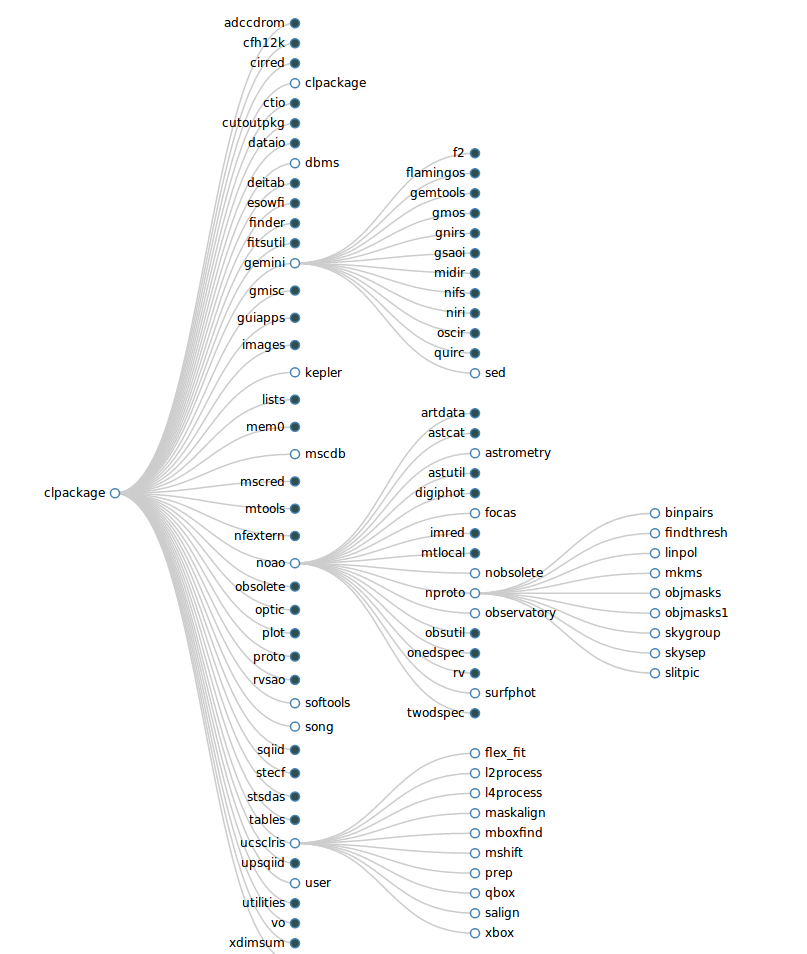
\includegraphics[width=.8\textwidth]{iraf_plot.png}
\end{figure}


\begin{figure}[h!]
\caption{Parallel lines chart to explore Baltimore city property taxes.} 
\centering
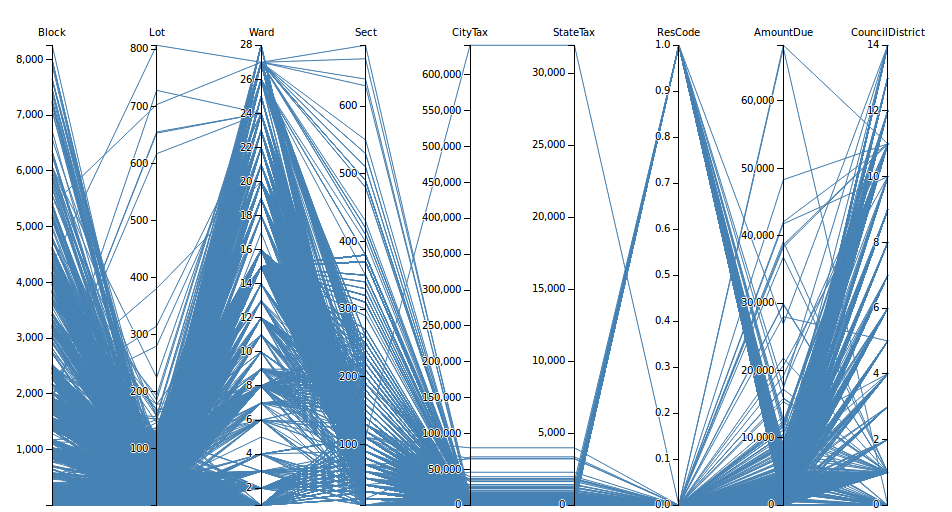
\includegraphics[width=.8\textwidth]{parallel_lines.png}
\end{figure}

\begin{figure}[h!]
\caption{Scatterplot matrix to explore Baltimore City salaries.} 
\centering
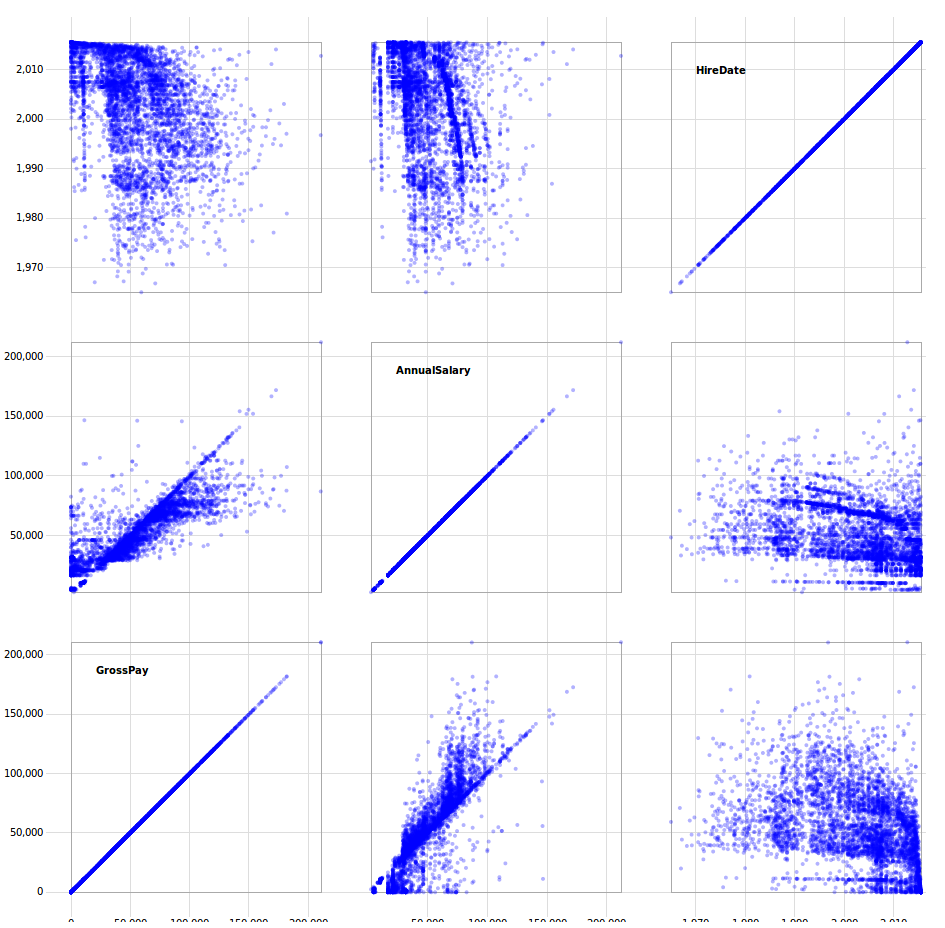
\includegraphics[width=.8\textwidth]{scatterplot.png}
\end{figure}


%%%%%%%%%%%%%%%%%%%%%%%%%%%%%%%%%%%%%%%%%%%%%%%%%%%%%%%%%%


\end{document}
